\section{ALOHA}
\marginnote{From ./AE-Specifications-ETH/standalone/Aloha.tex}

This section compares the classical ALOHA protocol with its improved variant, Slotted ALOHA, highlighting differences in their design, collision behavior, and efficiency.

\subsection{Introduction}

The \textbf{ALOHA protocol}\sidenote{Developed in the late 1960s at the University of Hawaii for radio communications} allows nodes to transmit packets at any time, leading to frequent collisions. 
\textbf{Slotted ALOHA}\sidenote{Introduced shortly after by Roberts in 1972}, in contrast, divides time into discrete slots, allowing transmissions only at the beginning of a slot, thereby reducing the chance of collisions.

\cite{Abramson1970, Kleinrock1975}

\subsection{Comparison Table}

\begin{table}[h]
\centering
\begin{tabular}{@{}lll@{}}
\toprule
\textbf{Feature} & \textbf{ALOHA} & \textbf{Slotted ALOHA} \\
\midrule
Time structure & Any time & Slot-aligned \\
Collision probability & High & Lower \\
Efficiency (max) & $\approx 18\%$ (1/2e) & $\approx 37\%$ (1/e) \\
Implementation complexity & Simple & Needs synchronization \\
Analogy & Random shouting & Timed shouting \\
\bottomrule
\end{tabular}
\caption{Key differences between ALOHA and Slotted ALOHA.}
\end{table}

\subsection{Visual Comparison}

Figure~\ref{fig:aloha-diagram} shows a visual comparison of packet transmissions and collisions in both protocols.

\begin{figure}[h]
\centering
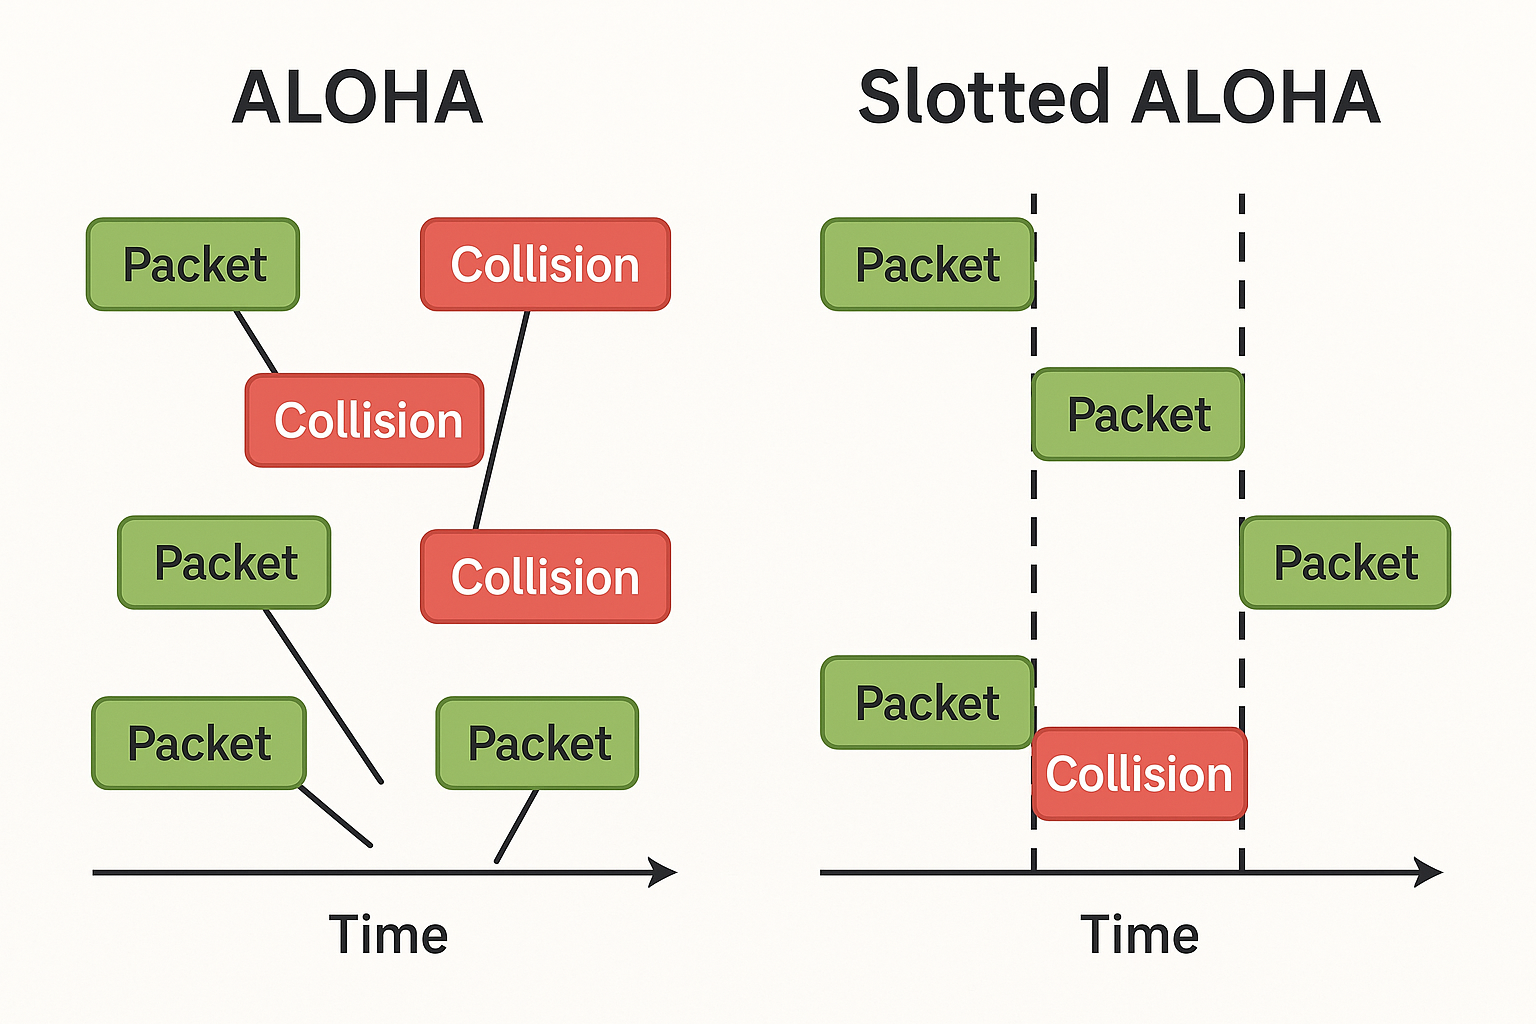
\includegraphics[width=0.8\linewidth]{../figures/aloha.png}
\caption{Collision behavior in ALOHA (left) vs. Slotted ALOHA (right).}
\label{fig:aloha-diagram}
\end{figure}

\subsection{Summary with Sidenotes}

\textbf{ALOHA} allows nodes to transmit without coordination,\sidenote{This freedom results in many partial collisions where packets overlap partially in time.} but suffers from a high collision probability.

\textbf{Slotted ALOHA} improves throughput by enforcing transmission only at predefined time slots,\sidenote{By waiting until the next time slot boundary, nodes avoid partial overlaps.} achieving almost twice the maximum throughput.

Overall, Slotted ALOHA introduces a modest increase in complexity but greatly improves network performance in high-load scenarios.\sidenote{Especially important for early satellite and Ethernet networks.}
